% =====================================================================================================
\section{Study 1: Strategic Play and Discrimination}\label{sec:study1}

\subsection{Design}
Study 1 is a complete randomised-block design with case as the block. Every one of the 48 main cases is played under all
$2\times3\times2\times2=24$ combinations of the prosecutor's objective (advocate, minister), the prosecutor's selection
rule (random, introspect, lookahead), the defence's selection rule (random, lookahead) and the defendant's type
(guilty, innocent), one game per cell, for \SoneNgames{} games in randomised run order. The design compares complete policy procedures. Within an objective, the rules use the same candidate-generation
protocol: lookahead versus random selection measures the effect of evaluating candidates by simulated replies,
and lookahead versus introspection compares explicit simulation with the model's direct choice. These contrasts
include the additional inference used by each selector. The objective factor changes both the prosecutor's goal
instruction and the lookahead utility, so its effect is not attributable to the utility formula alone. Crossing
these factors with defendant type measures discrimination, while the defence factor tests the effect of a
countervailing selection policy with the scoring access described in \cref{sec:materials}.

\paragraph{Hypotheses and analysis.} The specified hypotheses H1--H6 and their contrasts are listed in
\cref{tab:confirm}; the primary outcome is the primary judge's soft probability of guilt after round~4 (0--100). Each
contrast is computed within case (averaging over the factors it does not name) and tested across the 48 cases with a
two-sided $t$-test, with Holm correction over the nine confirmatory hypotheses of both studies. Bootstrap and sign-flip
results are in \cref{app:prereg}. The second validation experiment supplied the variance estimates for power calculations: with 48 cases the minimum detectable effect at 80\% power
is about 1.3 points for H1 and H3, 0.5 points for H5 and 0.8 points for H2, while H4 was expected to be underpowered.

\subsection{Results}

\paragraph{Manipulation and measurement checks.}
The recorded conversations distinguished defendant types on average. Under the primary judge,
guilty twins ended \TypeEffect{} points above their innocent twins, and in \PAUCOverall\% of cases the guilty twin
was judged guiltier (averaging over the 12 cells). The verdict-game rule convicted \ConvRateG\% of guilty and
\ConvRateI\% of innocent defendants. All six judges discriminated in the same direction (\cref{tab:judges}); DeepSeek
did so most strongly (\TypeEffectE{}). Both judges evaluated at every round showed \emph{examination drift}
(\cref{fig:drift}): the primary judge's probability of guilt rose from \DriftAGZero{} before the examination to
\DriftAGFour{} (guilty) and \DriftAIFour{} (innocent) after four rounds, as in the validation experiments. This pattern is consistent with an incriminating effect of
continued examination, but the design does not isolate question count from the content of the exchanges. The primary judge is
close to deterministic: re-querying 200 random prefixes gave $r=\RetestAR$ with a mean absolute difference of
\RetestAMAD{} points and \RetestAVerdict\% verdict agreement. DeepSeek, which reports stated probabilities, was
noisier ($r=\RetestER$, \RetestEMAD{} points).

\begin{table}[t]
\centering\small
\caption{Confirmatory hypothesis tests (Study 1: H1--H6, outcome = primary judge's probability of guilt after
round 4, in points; Study 2: H7--H9, immediate outcome). Estimates are means of within-case contrasts over 48 cases;
$d_z$ is the mean divided by the SD of case-level contrasts; $p_{\text{Holm}}$ adjusts across all nine hypotheses.}
\label{tab:confirm}
\begin{tabular}{@{}llrlrrr@{}}\toprule
 & Contrast & Estimate & 95\% CI & $d_z$ & $p$ & $p_{\text{Holm}}$\\\midrule
H1 & Strategic advantage: advocate lookahead $-$ random & +2.27 & [+1.64, +2.89] & +1.05 & \ensuremath{<}0.001 & \ensuremath{<}0.001\\
H2 & Simulation vs introspection (advocate) & +0.82 & [+0.26, +1.39] & +0.42 & 0.005 & 0.010\\
H3 & Advocate lookahead $-$ random, innocent defendants & +1.70 & [+0.84, +2.56] & +0.57 & \ensuremath{<}0.001 & \ensuremath{<}0.001\\
H4 & Discrimination: minister $-$ advocate (lookahead) & \ensuremath{-}0.33 & [\ensuremath{-}1.68, +1.01] & \ensuremath{-}0.07 & 0.624 & 0.624\\
H5 & Defence lookahead $-$ random & \ensuremath{-}2.26 & [\ensuremath{-}2.57, \ensuremath{-}1.95] & \ensuremath{-}2.15 & \ensuremath{<}0.001 & \ensuremath{<}0.001\\
H6 & Transfer gap: planner's judge $-$ held-out judges & +1.20 & [+0.48, +1.93] & +0.48 & 0.002 & 0.005\\
H7 & Move value: planner pick $-$ random (immediate) & +2.91 & [+2.38, +3.45] & +1.59 & \ensuremath{<}0.001 & \ensuremath{<}0.001\\
H8 & Crossover: matched $-$ mismatched (SD units) & +0.65 & [+0.38, +0.92] & +0.71 & \ensuremath{<}0.001 & \ensuremath{<}0.001\\
H9 & Dose-response slope per doubling of $k$ & +0.95 & [+0.78, +1.13] & +1.57 & \ensuremath{<}0.001 & \ensuremath{<}0.001\\
\bottomrule\end{tabular}

\end{table}

\paragraph{Confirmatory tests.}
\Cref{tab:confirm} reports the nine specified tests. Lookahead raised the advocate's probability of guilt by
\HOneCI{} points (H1, $d_z={}$\HOnedz, $p_{\text{Holm}}$\,\HolmHOne). This is a large and consistent standardised effect, but modest in absolute terms. In verdict terms it adds
\ConvAdvLook{} percentage points to the conviction rate. Explicit simulation exceeded introspective choice under
the same candidate-generation protocol by \HTwoCI{}
(H2), so modelling the opponent and the judge adds value beyond the LLM's unaided judgement. Lookahead raised the
probability of guilt for \emph{innocent} defendants by \HThreeCI{} (H3). There was no clear difference in discrimination
between minister and advocate objectives under lookahead (H4: \HFourCI{}; the 90\% interval \TostHFour{} contains zero but also effects of more than one point
in favour of the advocate, so this is an inconclusive null rather than evidence of equivalence). A lookahead defence
changed the probability of guilt by \HFiveCI{} (H5, $d_z={}$\HFivedz). The strategic advantage was \HSixCI{} points larger
when measured by the judge the planner had modelled than when averaged over the five held-out judges (H6).

\begin{figure}[t]
\centering
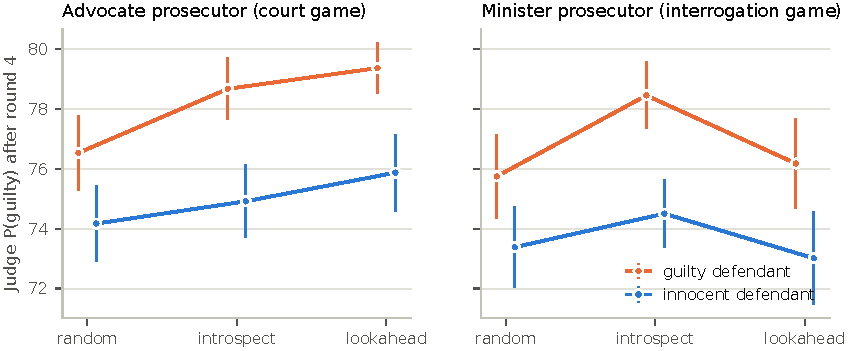
\includegraphics[width=\linewidth]{figs/s1_cells.pdf}
\caption{Study 1: primary judge's probability of guilt after round 4 by prosecutor objective, selection rule and
defendant type, averaged over the defence factor. Error bars are 95\% intervals of cell means across the 48 cases. These intervals describe cell means; uncertainty in a paired contrast also depends on covariance between cells
and should be read from \cref{tab:confirm}.}
\label{fig:cells}
\end{figure}

\paragraph{Discrimination and conviction.}
\Cref{fig:cells} decomposes the effect by defendant type. For the advocate, lookahead raised the probability of guilt
for guilty defendants by \AdvLookG{} and for innocent defendants by \AdvLookI{}, so it improved discrimination by
\DiscChgAdvLook{} points: strategy here is partly informative. In verdict terms, it raised convictions of guilty
defendants by \ConvAdvLookG{} percentage points and of innocent defendants by \ConvAdvLookI{} ($p=\ConvAdvLookIP$).
Under the post hoc threshold classifier ($P\ge80$), wrongful convictions rose by \ConvThrAdvLookI{} points
($p=\ConvThrAdvLookIP$). The court-game objective therefore buys more correct convictions at the price of more
wrongful ones, which is exactly the trade-off a strategic interrogator in a Turing test would face between catching
machines and flagging humans. Under the minister objective, the estimated lookahead effect was small and uncertain (\MinLook{}). It did not, however, buy better truth-tracking: the minister's discrimination
change under lookahead was \DiscChgMinLook{}. The arm that improved discrimination most reliably was introspection, by
\DiscChgAdvIntr{} (advocate) and \DiscChgMinIntr{} (minister) points.

\paragraph{Evidence disclosure.}
An exploratory content analysis of all 4,608 questions (coded by DeepSeek-V4-Flash; 600 double-coded by GPT-4o-mini)
shows what the arms do differently. Disclosure of withheld evidence was coded reliably ($\kappa=\KappaDisc$). In round
1, random selection disclosed it in \DiscROneRandAdv\% of advocate games. Introspection raised this by
\DiscROneAdvIntr{} percentage points and advocate lookahead by \DiscROneAdvLook{}, whereas minister lookahead did not
change it (\DiscROneMinLook{}). Across arms, early confrontation with the withheld record coincides with better discrimination: the three arms that
disclose more in round 1 are the three arms whose discrimination improved, and the one arm that did not disclose more
did not improve. This is correlational across four arms, not a mediation analysis. A plausible mechanism is that a
guilty defendant whose cover story is contradicted by a record must improvise, whereas an innocent one simply
explains it. Notably, this runs against the classical SUE advice to elicit an account before disclosing; we
conjecture that LLM liars do not commit to a story early enough for late disclosure to pay off, a hypothesis for
future work. The minister's planner did not move towards confrontation, consistent with its simulated suspects
(which see only the public file) not reproducing how real guilty and innocent defendants differ
\MinisterSignalText{}. Fabricated factual claims were rarer and coded less reliably
($\kappa=\KappaFab$). They grew from \FabRoundOne\% of round-1 to \FabRoundFour\% of round-4 questions and were
more common for advocates (\FabAdv\% vs \FabMin\%), but lookahead did not detectably select for them (advocate:
\FabAdvLook{} percentage points, $p=\FabAdvLookP$). Nearly all questions (\RateLead\%) were leading, so that feature was
uninformative.

\begin{figure}[t]
\centering
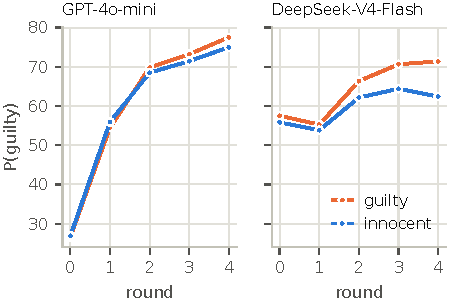
\includegraphics[width=0.56\linewidth]{figs/s1_drift.pdf}
\caption{Examination drift: mean probability of guilt by round for the two judges that scored every round (the
planner's judge and DeepSeek), in the random-versus-random cells of Study 1. Guilty (orange) and innocent (blue) twins start from the same prior, because
the court's file is identical, and separate as the examination proceeds, while both drift upwards.}
\label{fig:drift}
\end{figure}

\paragraph{Strategic interaction.}
The defence's lookahead changed the conviction rate by \ConvDef{} percentage points. It did not neutralise the prosecutor's
advantage: the advocate's gain from lookahead was \AdvLookDefRand{} against a random defence and \AdvLookDefLook{}
against a lookahead defence (interaction \PxD{}). Strategies on the two sides are approximately additive. In the estimated
$3\times2$ zero-sum matrix with final guilt score as the payoff (\cref{tab:meta}), lookahead is strictly dominant
for both players. This matrix has the unique equilibrium (lookahead, lookahead), with value \MetaValue{}, close to
the score under random selection on both sides. These are properties of the estimated surrogate matrix; they do
not establish dominance in the full verdict game or account for uncertainty in the matrix entries.

\begin{table}[t]
\centering\small
\caption{Estimated policy meta-game: mean final probability of guilt (primary judge) by prosecutor and defence selection rule, advocate
objective. NE = Nash-equilibrium weights of the zero-sum game in which the prosecutor maximises and the defence
minimises this payoff.}\label{tab:meta}
\begin{tabular}{@{}lccc@{}}\toprule
 & \multicolumn{2}{c}{Defence} & \\\cmidrule(lr){2-3}
Prosecutor (advocate) & random & lookahead & NE weight\\\midrule
random & 76.4 & 74.3 & 0.00\\
introspect & 77.7 & 75.9 & 0.00\\
lookahead & 78.7 & 76.5 & 1.00\\
NE weight (defence) & 0.00 & 1.00 & \\
\bottomrule\end{tabular}

\vspace{0.8em}
\caption{Judge panel scoring the same 1,152 transcripts: final probability of guilt (mean, SD), discrimination between
twins, and the advocate's lookahead advantage with its $p$-value. ``Soft'' = renormalised mean over returned
integer tokens, with a stated-score fallback; ``stated'' = the number the judge wrote.}\label{tab:judges}
\begin{tabular}{@{}llrrlll@{}}\toprule
Judge & $p$ & Mean & SD & Guilty $-$ innocent & Lookahead $-$ random (adv.) & $p$\\\midrule
GPT-4o-mini & soft & 75.9 & 5.2 & +3.2 [+2.7, +3.6] & +2.3 [+1.6, +2.9] & \ensuremath{<}0.001\\
Llama-3.3-70B & soft & 83.4 & 4.2 & +2.0 [+1.5, +2.5] & +0.6 [+0.1, +1.1] & 0.018\\
Gemini-2.5-FL & stated & 75.3 & 6.3 & +2.5 [+1.8, +3.2] & +1.5 [+0.4, +2.5] & 0.007\\
Claude-Haiku-5.5 & stated & 77.6 & 7.9 & +3.8 [+3.0, +4.7] & +1.0 [\ensuremath{-}0.3, +2.3] & 0.112\\
DeepSeek-V4-Flash & stated & 66.7 & 15.3 & +8.9 [+7.3, +10.5] & +1.4 [\ensuremath{-}0.5, +3.4] & 0.134\\
Mistral-Small-3.2 & stated & 78.9 & 11.9 & +5.9 [+4.0, +7.8] & +0.8 [\ensuremath{-}0.9, +2.5] & 0.359\\
\bottomrule\end{tabular}

\end{table}

\paragraph{Transfer across evaluators.}
Holding the implemented policies fixed, we scored the same 1,152 transcripts with six evaluators. Final scores
refer to forced continuation; first-decisive-verdict outcomes use \cref{prop:decouple}.
The advocate's lookahead advantage was \AdvLookJudgeA{} under the planner's own judge, and \AdvLookJudgeB{},
\AdvLookJudgeC{}, \AdvLookJudgeD{}, \AdvLookJudgeE{} and \AdvLookJudgeF{} under Llama, Gemini, Haiku, DeepSeek and
Mistral (\cref{fig:transfer}). It is positive under every judge but roughly half as large, consistent with
specialisation to the modelled classifier. Differences in evaluator scales also affect this comparison; Study 2
examines evaluator dependence through a standardised crossover.

\paragraph{Sensitivity to judge instructions.}
Re-scoring the same transcripts with a guilt-leaning instruction (``treat vague, evasive or inconsistent answers
about the evidence as strong indications of guilt'') raised the mean final probability from \PfinalMeanA{} to \GLMean{} and the
conviction rate from \NeutralConv\% to \GLConv\%. Under that instruction \GLConvI\% of innocent defendants were
convicted. It also halved the strategic advantage (\GLHOne{}) and shrank discrimination (\GLType{}). A single sentence
in the classifier's prompt produced larger changes in these outcomes than the tested player strategies.

\begin{figure}[t]
\centering
\begin{minipage}[t]{0.49\linewidth}\centering
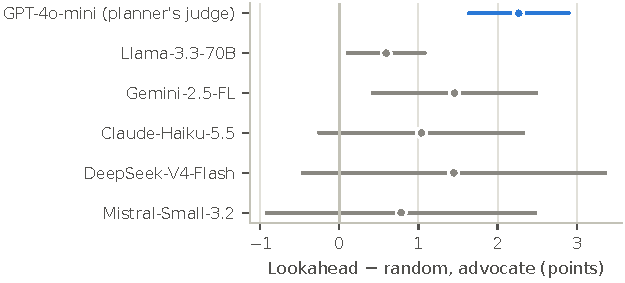
\includegraphics[width=\linewidth]{figs/s1_transfer.pdf}
\caption{Advocate lookahead advantage evaluated by each judge on identical transcripts (95\% CIs). The planner modelled
GPT-4o-mini.}\label{fig:transfer}
\end{minipage}\hfill
\begin{minipage}[t]{0.49\linewidth}\centering
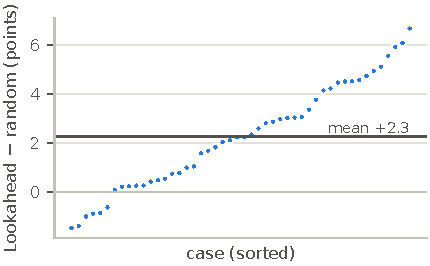
\includegraphics[width=\linewidth]{figs/s1_cases.pdf}
\caption{Case-level advocate lookahead advantage (each dot one case, averaged over defence and type), sorted.}\label{fig:cases}
\end{minipage}
\end{figure}

\paragraph{Heterogeneity across cases.}
The advantage was positive in \CasesPositive{} of \CasesTotal{} cases (\cref{fig:cases}). A random-slope model puts
the between-case standard deviation of the effect at $\hat\tau=\HetTau$ points. The model-based interval
$\hat\beta\pm1.96\hat\tau$ is \HetPI{} for the latent effect in a comparable new synthetic case, where
$\hat\beta$ is the fitted mean effect. It conditions on the fitted parameters and omits uncertainty in their estimation.
Repeated runs of a single case would estimate simulation variability but not this between-case variation.
